\section{Experiments}
\subsection{Implementation}

We follow Cellpose~\cite{stringer2021cellpose} and utilize their U-Net architecture and the data to pretrain the network on a Titan Xp GPU for 500 iterations with a batch size of 8. Since our approach is considered a test-time adaptation approach, we adapt to test instances from the test split of various benchmarks we evaluate in this manuscript. We use SGD with the learning rate of 0.01, momentum 0.9, weight decay of 0.00001, and batch size of 2. We take square patches of size $h=w=112$, with a minimum overal of 48 during evaluation, and nominal cell size $m_n = 30$. Hyperparameters for adaptation losses are $\lambda_1 = \lambda_2 = 1.0$.  Following ~\cite{keaton2023celltranspose}, we set other hyperparameters as: $|\mathcal{N}_i|=20, \tau=0.1$, and $\theta=0.05$.

\subsection{Evaluation Metrics}
Following Cellpose~\cite{stringer2021cellpose}, we quantify our predictions by matching our predicted masks with the ground truth masks, and whichever provides the highest IoU becomes the pair we consider as true positive (TP). The masks without any valid matches are false positives (FP), and the ground truth masks without any valid matches are considered false negatives (FN). With these predictions defined, we compute the standard average precision metric AP for each image and then average it as defined below:
\begin{equation}
    AP = \frac{TP}{TP+FP+FN}
\end{equation}   
We also compute the F1 score which is given by:
\begin{equation}
    F1 = \frac{TP}{TP+\frac{1}{2}(FP+FN)}
\end{equation} 
\subsection{Datasets}
We choose Cellpose~\cite{stringer2021cellpose} Generalist dataset as our source data and \textbf{TissueNet}~\cite{TissueNet} data splits as our various domains we want to adapt to. TissueNet~\cite{TissueNet} collects tissue data (i.e., Breast, GI, Immune, Pancreas, etc.) from many platforms (i.e., CyCIF, CODEX, Vectra, MIBI, etc. ). We adapt to each of these specific domains separately in our experiments. In \Cref{tab:tn1,tab:tn2}, we show relative improvement over various dataset splits within TissueNet. The left portion describes the platform type and the right describes the tissue type. In each case, we show that we improve over the baseline. For example, for Codex-Pancreas, we improved from 0.717 to 0.742 in just one backward pass without any target labels or source data. We also present qualitative evaluation of our approach in \Cref{fig:qual}. In each of the cases illustrated, we can observe relatively low number of false positives and false negatives in the adapted version compared to the baseline.

\begin{table}
    
    \caption{Comparative analysis on various splits of TissueNet. We show improvement with test-time adaptation. }
    \label{tab:tn1}
    \scalebox{0.8}{
\begin{tabular}{c|cc|cc|cc}
    CP $\rightarrow$ TN  & \multicolumn{2}{l|}{Codex-Pancreas} & \multicolumn{2}{l|}{CyCIF-Immune} & \multicolumn{2}{l}{MIBI-Breast} \\
                            & {AP}             & F1                    & {AP}             & F1                    & {AP}             & F1                    \\ 
\hline
Cellpose                  & {0.717}          & 0.836                 & {0.476}          & 0.640                 & {0.228}          & 0.346                 \\ 
Cellpose-tta              & {\textbf{0.742}} & \textbf{0.853}        &{\textbf{0.501}} & \textbf{0.661}        & {\textbf{0.239}} & \textbf{0.361}        \\ 
CellTranspose             &                &  &               & & &  \\
\end{tabular}
    }
\end{table}

\begin{table}
    
    \caption{Comparative analysis on various splits of TissueNet. We show improvement with test-time adaptation. }
    \label{tab:tn2}
    \scalebox{0.8}{
\begin{tabular}{c|cc|cc|cc}
    CP $\rightarrow$ TN  & \multicolumn{2}{l|}{Mixif-GI} & \multicolumn{2}{l|}{Vectra-Immune} & \multicolumn{2}{l}{Vectra-Breast} \\
                            & {AP}             & F1                    & {AP}             & F1                    & {AP}             & F1                    \\ 
\hline
Cellpose                  & {0.355}          & 0.527                 & {0.629}          & 0.776                 & {0.574}          & 0.745                 \\ 
Cellpose-tta              & {\textbf{0.373}} & \textbf{0.545}        &{\textbf{0.631}} & \textbf{0.777}        & {\textbf{0.583}} & \textbf{0.751}        \\ 
CellTranspose             &                &  &               & & &  \\
\end{tabular}
    }
\end{table}


\begin{figure}
    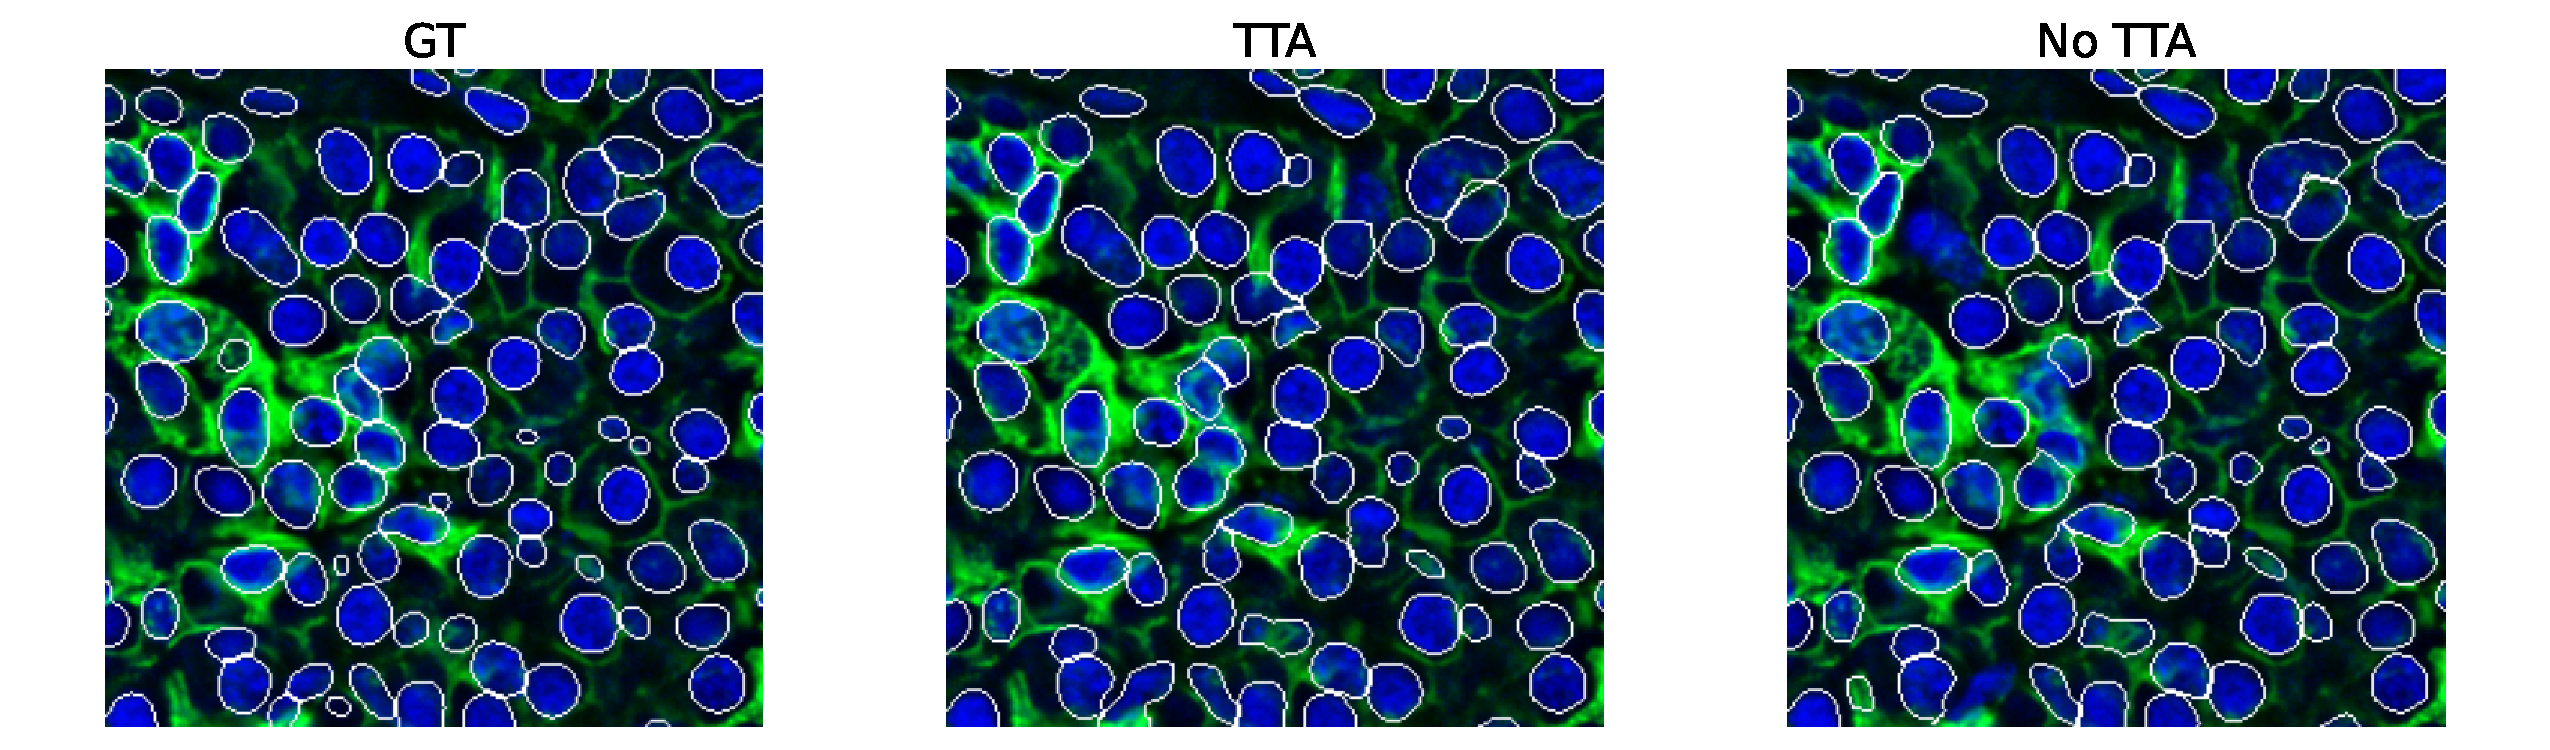
\includegraphics[width=8.75cm]{figs/1.pdf}
    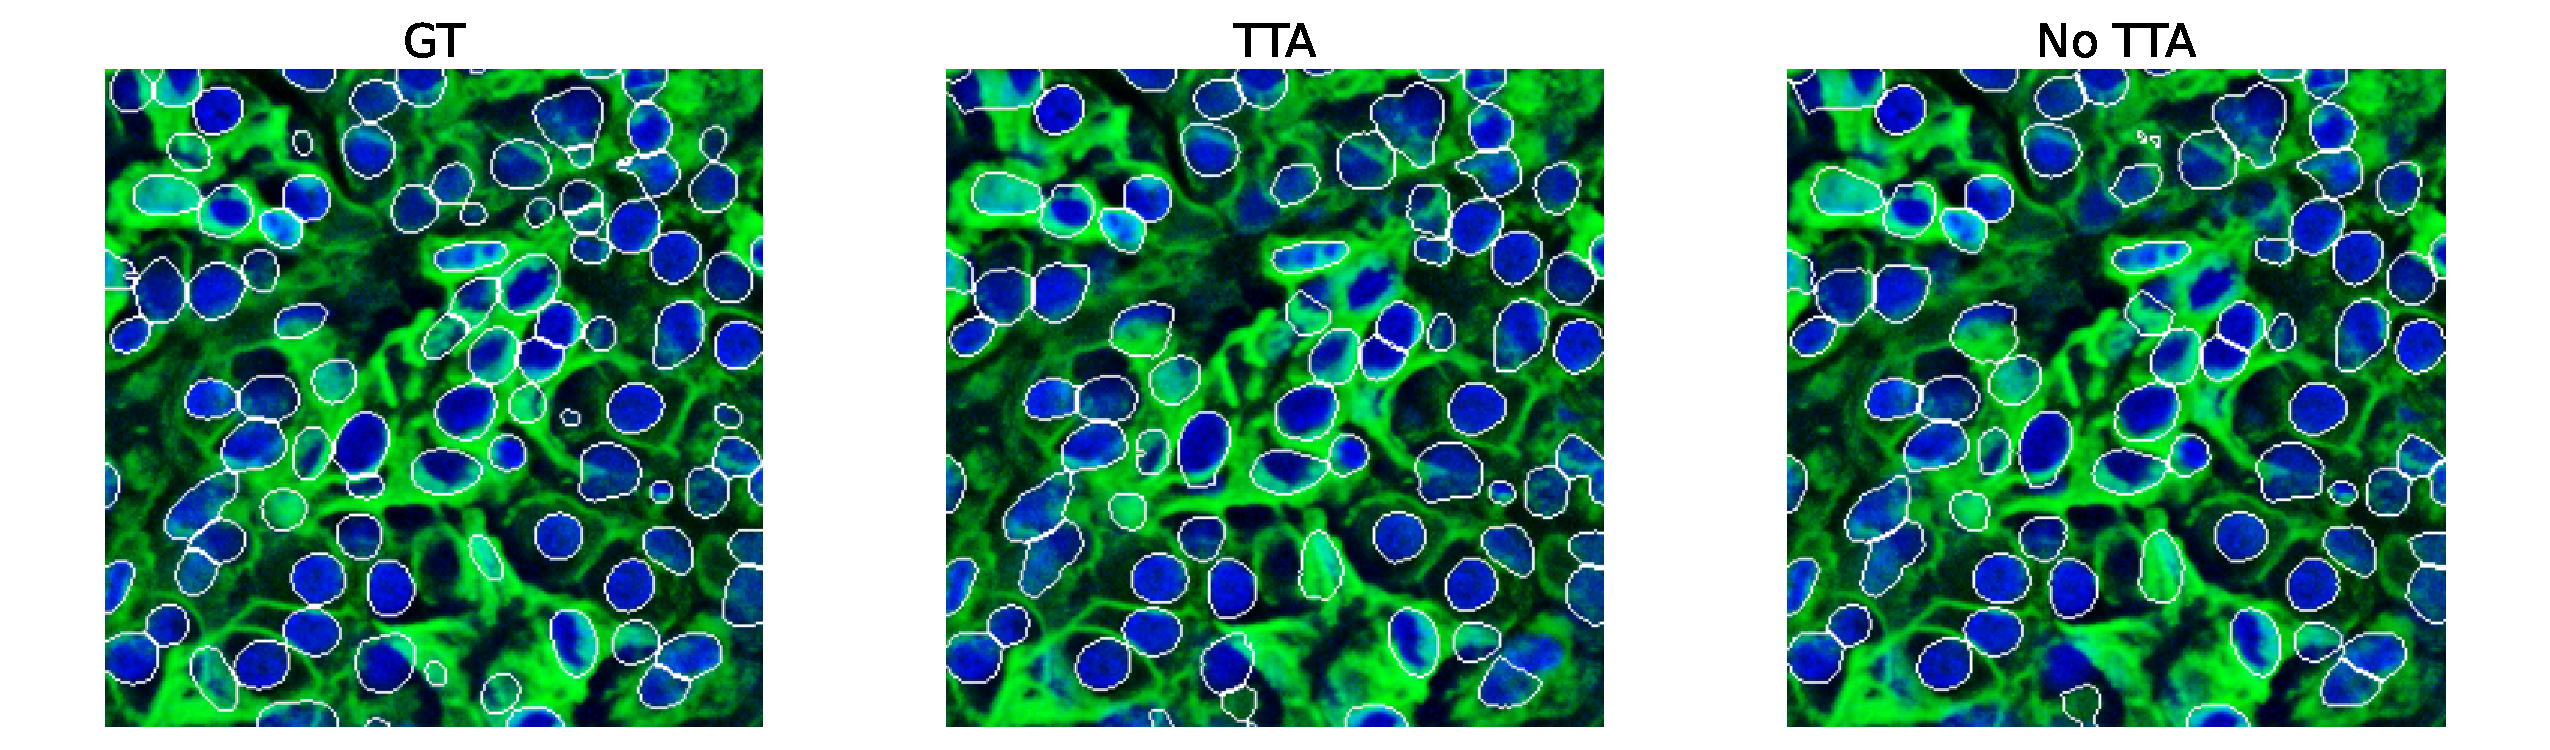
\includegraphics[width=8.75cm]{figs/43.pdf}
    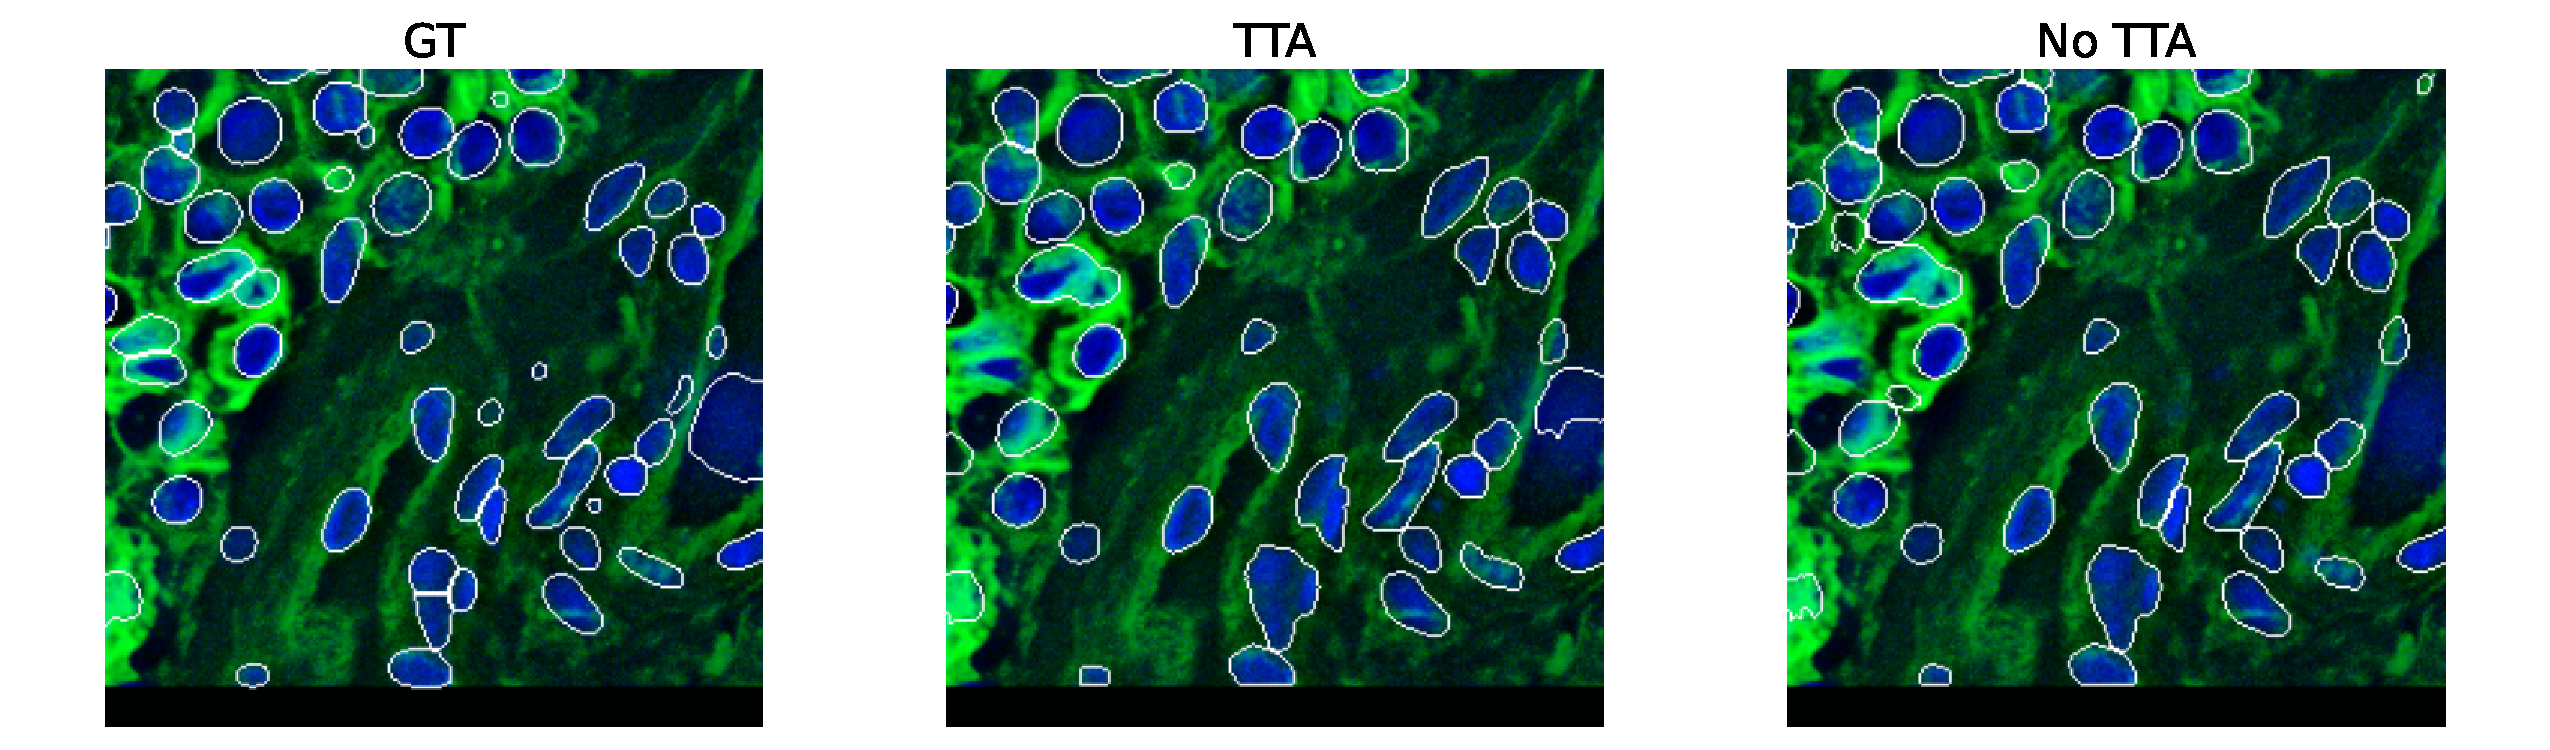
\includegraphics[width=8.75cm]{figs/45.pdf}
    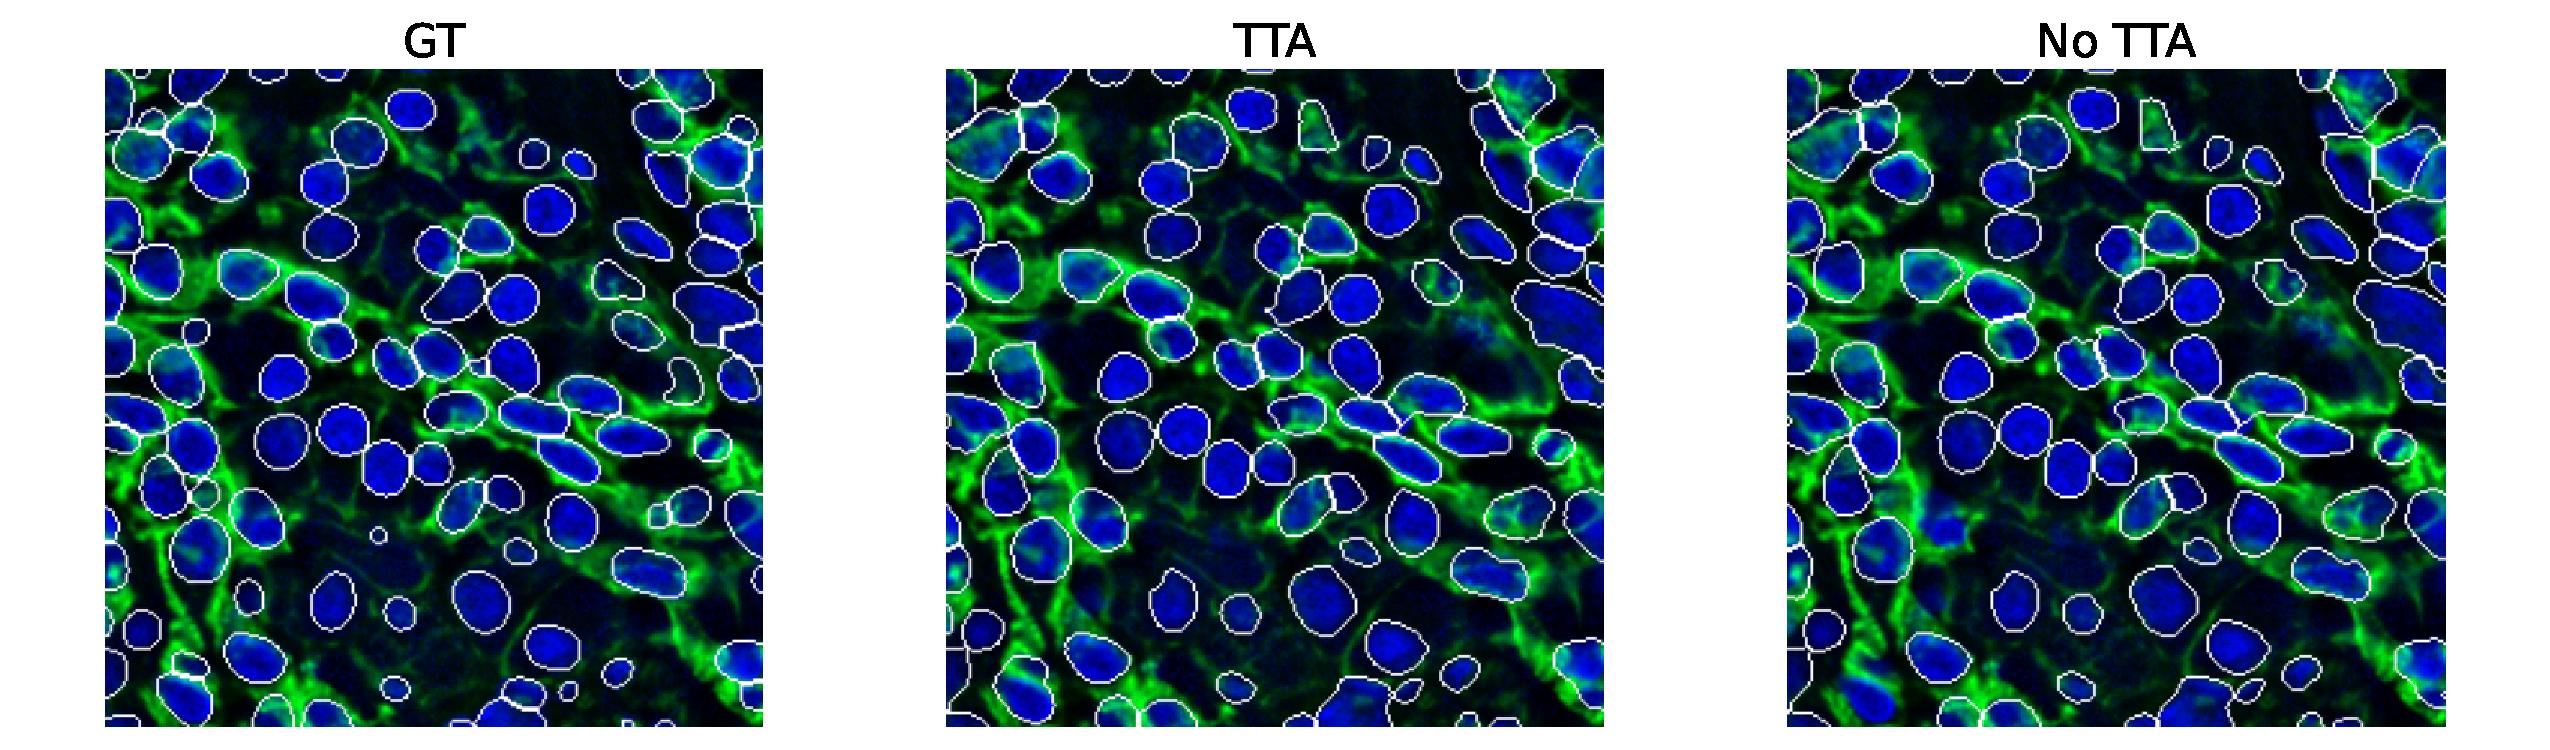
\includegraphics[width=8.75cm]{figs/55.pdf}
    \caption{\textbf{Illustating TTA results on Codex-Pancreas dataset from TissueNet against the ground truth and the baseline.} In each of the cases illustrated, we can observe relatively low number of false positives and false negatives in the adapted version compared to the baseline.}
    \label{fig:qual}
\end{figure}